\chapter{Planificación y Seguimiento}

En este capítulo detallaramos la planificación de cada una de las iteraciones que hemos hecho, así como el seguimiento realizado. La elaboración de este proyecto se llevó a cabo durante dos años, comenzando en junio de 2014 y teniendo un par de parones durante varios meses (desde septiembre de 2014 hasta enero de 2015 y desde mayo de 2015 hasta septiembre del mismo año). 
Por lo tanto, los periodos de actividad serían los siguientes:

\begin{itemize}
  \item Desde junio del año 2014 hasta septiembre del 2014 (3 meses).
  \item Desde enero de 2015 hasta mayo del mismo año (4 meses).
  \item Desde septiembre del 2015 hasta abril de 2016 (8 meses).
\end{itemize}

En las próximas secciones hablaremos de lo que hemos desarrollado durante estos tres periodos de tiempo y las iteraciones seguidas en los mismos.

Cabe destacar que todos los datos y tareas mostradas a continuación están realizadas de forma lineal, dado que solamente disponemos de un recurso.

\section{Junio 2014 - Septiembre 2014}

Este periodo comienza el 4 de junio, que es cuando se nos comenta la posibilidad de realizar este proyecto, y termina el 28 de septiembre, por lo que consta de un total de 17 semanas. Hay que tener en cuenta que durante parte de este verano (desde agosto) es cuando me mudé a Holanda y empiecé mi \textit{internship}, por lo que las jornadas en días laborables solamente constaban de una o dos horas y alrededor de 8/9 horas durante los fines de semana.

Sumando todo el tiempo empleado durante estas semanas se calcula que se han empleado 285 horas en total.

Durante este tiempo nos centramos en recabar información general para poder empezar el proyecto con buen pie, así como la implementación de los mapas y habitaciones.

\subsection{Primera iteración: Análisis de requisitos generales, diseño genérico y preparación y configuración de los elementos necesarios para el comienzo de la implementación}

Desde el 4 de junio hasta el 29 de junio.

\paragraph{Análisis de requisitos generales} Al desarrollar un proyecto enfocado a una parte de la población de la que no formas parte, es muy importante documentarse sobre todos los aspectos que hay que tener en cuenta e intentar ponerse en su piel (por ejemplo usar las herramientas que utilizan diariamente para recabar ideas).
Àsí mismo, desarrollar un videojuego puede llegar a ser una tarea infinita, dado que nuevas características o ideas que añadir es algo que sucede casi diaremente. Aprender sobre lo básico del género y poner límites es fundamental para centrar los pocos recursos que tenemos en crear lo completamente necesario.

\paragraph{Diseño genérico del juego a implementar} Crearemos el primer diseño genérico que nos dará una idea sobre lo que tendremos que realizar y nos guiará sobre el proceso de creación del juego. Este primer boceto cambiará a medida que querramos añadir nuevos elementos y querramos especificar más otros.

\paragraph{Búsqueda de bibliotecas que se adapten a nuestros requisitos} Hay varias bibliotecas con las que se puede crear una interfaz gráfica sencilla como la de Rogue, pero todas ellas tienen sus ventajas e inconvenientes. Debemos de averiguar cuál de ellas es la más adecuada para nuestro caso.

\paragraph{Creación y configuración del ambiente de desarrollo para poder empezar la implementación} Al empezar un nuevo proyecto debemos de crear un repositorio en git, instalar todo el software necesario y preparar lo básico para que podamos empezar a programar sin encontrarnos con ninguna dificultad a posteriori.

\subsection{Tareas y seguimiento}

La descomposición de las tareas es la siguiente:

\begin{enumerate}[label=\bfseries WBS 1.\arabic*]
  \item Análisis de requisitos generales
    \begin{enumerate}[label=\bfseries WBS 1.1.\arabic*]
      \item Estudio de herramientas para invidentes.
      \item Estudio de los elementos del género \textit{roguelike}.
      \item Analizar los elementos encontrados y especificación de lo que queremos en nuestro caso.
    \end{enumerate}
  \item Diseño genérico del juego a implementar.
  \item Búsqueda de bibliotecas que se adapten a nuestros requisitos.
  \item Creación y configuración del ambiente de desarrollo para poder empezar la implementación.
\end{enumerate}

Para la realización de todas estas tareas se planificaron 65 horas en total. Esta estimación se cumplió, por lo que al final de la iteración todas las tareas habían sido realizadas. Ver la figura ~\ref{fig:sec1it1}

\begin{figure}
    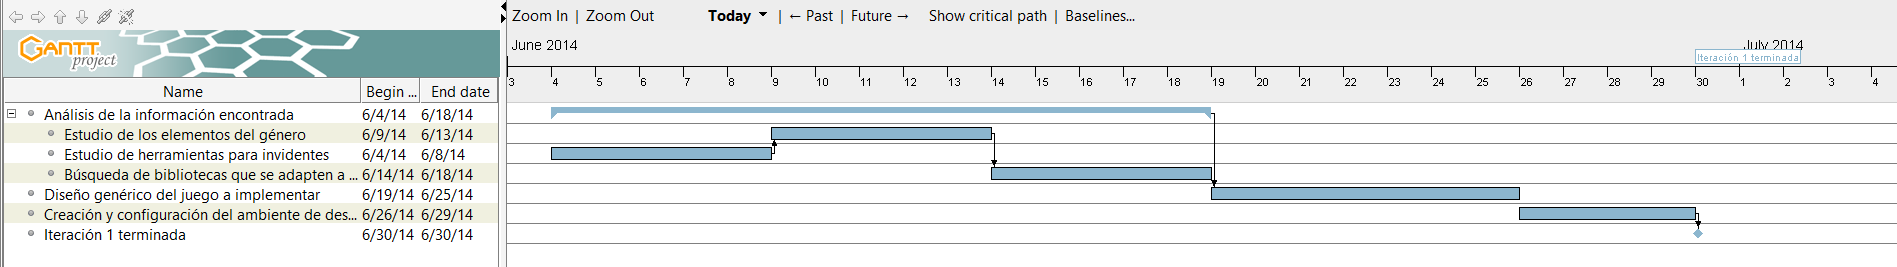
\includegraphics[width=\textwidth,height=\textheight,keepaspectratio]{./img/sec1it1.png}
  \caption{Diagrama de Gantt de la primera iteración de la primera etapa}
  \label{fig:sec1it1}
\end{figure}